% !TeX TXS-program:compile = txs:///arara
% arara: pdflatex: {shell: no, synctex: no, interaction: batchmode}
% arara: pdflatex: {shell: no, synctex: no, interaction: batchmode}

\documentclass[11pt,a4paper]{ltxdoc}
\usepackage{bera}
\usepackage{inconsolata}
\usepackage[T1]{fontenc}
\usepackage[scale=0.875]{cabin}
\usepackage{randintlist}
\usepackage{fancyvrb}
\usepackage{fancyhdr}
\usepackage{tabularray}
\usepackage{fontawesome5}
\fancyhf{}
\renewcommand{\headrulewidth}{0pt}
\lfoot{\sffamily\small [randintlist]}
\cfoot{\sffamily\small - \thepage{} -}
\rfoot{\hyperlink{matoc}{\small\faArrowAltCircleUp[regular]}}
\usepackage{hologo}
\providecommand\tikzlogo{Ti\textit{k}Z}
\providecommand\TeXLive{\TeX{}Live\xspace}
\let\TikZ\tikzlogo

\usepackage{hyperref}
\urlstyle{same}
\hypersetup{pdfborder=0 0 0}
\usepackage[margin=2cm]{geometry}
\setlength{\parindent}{0pt}
\def\TPversion{0.1.4}
\def\TPdate{05/05/2025}
\usepackage{tcolorbox}
\usepackage{pgffor}
\tcbuselibrary{breakable,skins,hooks,listingsutf8}
%\usepackage{soul}
%\sethlcolor{lightgray!25}

\lstset{
	language=[LaTeX]TeX,%
	basicstyle=\ttfamily,%
	keywordstyle={\color{blue}},%
	classoffset=0,%
	keywords={},%
	alsoletter={-},%
	keywordstyle={\color{blue}},%
	classoffset=1,%
	alsoletter={-},%
	morekeywords={randintlist},%
	keywordstyle={\color{violet}},%
	classoffset=2,%
	alsoletter={-},%
	morekeywords={\randintlist,\getitemfromrandintlist},%
	keywordstyle={\color{green!50!black}},%
	classoffset=3,%
	morekeywords={min,max,nb,seed,sort,sep,repeat,exclude},%
	keywordstyle={\color{orange}}
}

\newtcblisting{DemoCode}[1]{%
	enhanced,width=\linewidth,%
	bicolor,size=title,%
	colback=cyan!10!white,%
	colbacklower=cyan!5!white,%
	colframe=cyan!75!black,%
	listing options={%
		breaklines=true,%
		breakatwhitespace=true,%
		style=tcblatex,basicstyle=\small\ttfamily,%
		tabsize=4,%
		commentstyle={\itshape\color{gray}},
		keywordstyle={\color{blue}},%
		classoffset=0,%
		keywords={\usepackage,\includegraphics,xstring,listofitems,tikz,calc,simplekv,graphicx,\readlist,\showitems,\xintFor,\xintSeq},%
		alsoletter={-},%
		keywordstyle={\color{blue}},%
		classoffset=1,%
		alsoletter={-},%
		morekeywords={randintlist},%
		keywordstyle={\color{violet}},%
		classoffset=2,%
		alsoletter={-},%
		morekeywords={\randintlist,\getitemfromrandintlist,\ListeRandint,\ExtraireEltListeRandint},%
		keywordstyle={\color{green!50!black}},%
		classoffset=3,%
		morekeywords={min,max,nb,seed,sort,sep,repeat,Min,Max,Nb,Graine,Sep,Tri,Repet,exclude,Exclure},%
		keywordstyle={\color{orange}}
	},%
	#1
}

\newtcbinputlisting\DemoCodeFile[1]{%
	enhanced,width=\linewidth,%
	bicolor,size=title,%
	colback=lightgray!10!white,%
	colbacklower=lightgray!5!white,%
	colframe=lightgray!75!black,%
	listing options={%
		breaklines=true,%
		breakatwhitespace=true,%
		style=tcblatex,
		basicstyle=\scriptsize\ttfamily,%
		tabsize=4,%
		commentstyle={\itshape\color{gray}},%
		lastline=246
	},%
	breakable,
	listing only,%
	listing file={#1}
}

\NewDocumentCommand\ShowCode{ m }{%
	\lstinline{#1}%
}

\begin{document}

\thispagestyle{empty}

\begin{center}
	\begin{minipage}{0.88\linewidth}
		\begin{tcolorbox}[colframe=yellow,colback=yellow!15]
			\begin{center}
				\renewcommand{\arraystretch}{1.25}%
				\begin{tabular}{c}
					{\Huge \texttt{randintlist}}\\
					\\
					{\LARGE Creating random integer number lists,} \\
					{\LARGE with multiple numbers or not,} \\
					{\LARGE sorted or not.} \\
					\\
					{\small \texttt{Version \TPversion{} -- \TPdate}}
				\end{tabular}
			\end{center}
		\end{tcolorbox}
	\end{minipage}
\end{center}

\begin{center}
	\begin{tabular}{c}
		\texttt{Cédric Pierquet}\\
		{\ttfamily c pierquet -- at -- outlook . fr}\\
		\texttt{\url{https://forge.apps.education.fr/pierquetcedric/packages-latex}} \\
	\end{tabular}
\end{center}

\hrule

\vfill

\begin{tcolorbox}[colframe=lightgray,colback=lightgray!5]
10 numbers, between 1 and 100, without repetition:

\hfill\randintlist[min=1,max=100,nb=10]{\mylist}\textcolor{red}{\mylist}\hfill~

The 5th value is:

\hfill\textcolor{blue}{\getitemfromrandintlist{\mylist}{5}}\hfill~
\end{tcolorbox}

\begin{tcolorbox}[colframe=lightgray,colback=lightgray!5]
10 numbers, between 1 and 100, without multiples of 5:

\hfill\randintlist[min=1,max=100,nb=10,exclude={5,10,15,20,25,30,35,40,45,50,55,60,65,70,75,80,85,90,95,100}]{\mylist}\textcolor{olive}{\mylist}\hfill~

The 9th value is:

\hfill\textcolor{purple}{\getitemfromrandintlist{\mylist}{9}}\hfill~
\end{tcolorbox}

\begin{tcolorbox}[colframe=lightgray,colback=lightgray!5]
15 numbers, between 1 and 20, with repetition:

\hfill\randintlist[min=1,max=20,nb=15,repeat]{\mylist}\textcolor{red}{\mylist}\hfill~

The last value is:

\hfill\textcolor{blue}{\getitemfromrandintlist{\mylist}{-1}}\hfill~
\end{tcolorbox}

\begin{tcolorbox}[colframe=lightgray,colback=lightgray!5]
6 sorted numbers, between 1 and 51, without repetition:

\hfill\randintlist[min=1,max=51,nb=6,sort=asc]{\mylist}ascending : \textcolor{red}{\mylist}\hfill~

\hfill\randintlist[min=1,max=51,nb=6,sort=des,sep=>]{\mylist}descending : \textcolor{red}{\mylist}\hfill~
\end{tcolorbox}

\vfill~

\hrule

\medskip

\emph{%
	1. The \textsf{luarandom} package do the same things, but with the obligation to compile with \hologo{LuaLaTeX}.
}

\emph{%
	2. The \textsf{tuple} package is so much better\ldots\ but I keep \texttt{randintlist}, without new features\ldots
}

\medskip

\hrule

\vspace*{5mm}

\pagebreak

\phantomsection

\hypertarget{matoc}{}

\tableofcontents

\vspace*{5mm}

%\hrule

\pagebreak

\section{Loading, useful packages}

In order to load \texttt{randintlist}, simply use:

\begin{DemoCode}{listing only}
\usepackage{randintlist}
\end{DemoCode}

Loaded packages are \texttt{ifthen}, \texttt{simplekv}, \texttt{listofitems}, \texttt{randomlist},  \texttt{xintexpr} and \texttt{xstring}.

\section{The Macros}

\subsection{Global usage}

Package \texttt{randintlist} supports the creation of random integer number lists where a number will appear only once or multiple times. Generated lists can te used with \texttt{listofitems}.

\hfill\textbf{All engines \TeX\ are compatible with this package.}\hfill~

\subsection{Generate the list}

\begin{DemoCode}{listing only}
%generate list
\randintlist[keys]{\macro}
\end{DemoCode}

Available keys are:

\begin{itemize}
	\item \ShowCode{min}: minimum value (default \ShowCode{1});
	\item \ShowCode{max}: maximum value (default \ShowCode{50});
	\item \ShowCode{nb}: number of values (default \ShowCode{6});
	\item \ShowCode{sep}: separator for the list (default \ShowCode{,});
	\item \ShowCode{sort}: sorting options, within \ShowCode{no/asc/dec} (default \ShowCode{no});
	\item \ShowCode{repeat}: boolean to authorize repeating values (default \ShowCode{false});
	\item \ShowCode{exclude}: list of excluded values (default \ShowCode{empty});
	\item \ShowCode{seed}: random seed value according to used packages (default \ShowCode{-}).
\end{itemize}

\begin{DemoCode}{}
%default values
\randintlist{\mylistA}\mylistA
\end{DemoCode}

\begin{DemoCode}{}
%10 between 1 and 50, with ascending
\randintlist[sort=asc,min=1,max=50,nb=10]{\mylistB}\mylistB
\end{DemoCode}

\begin{DemoCode}{}
%15 between 1 and 50, with ascending and repetitions allowed
\randintlist[sort=asc,min=1,max=50,nb=15,repeat]{\mylistC}\mylistC
\end{DemoCode}

\begin{DemoCode}{}
%15 between 1 and 50, without multiples of 5
\randintlist[%
	sort=asc,min=1,max=50,nb=15,repeat,%
	exclude={5,10,15,20,25,30,35,40,45,50}]%
	{\mylistC}\mylistC
\end{DemoCode}

\begin{DemoCode}{}
%list used with listofitems
\randintlist{\mylistD}\mylistD\par
\readlist*\mylistused{\mylistD}\showitems{\mylistused}\par
\mylistused[1]; \mylistused[-1]
\end{DemoCode}

\subsection{Accessing elements}

\begin{DemoCode}{listing only}
%accessing item
\getitemfromrandintlist[separator]{\macro}{index}[\macrores]
\end{DemoCode}

\begin{DemoCode}{}
%with default keys
\randintlist{\mylistE}raw list: \mylistE\par
items list:\par
\xintFor* #1 in {\xintSeq{1}{6}}\do{\getitemfromrandintlist{\mylistE}{#1}\par}
first element: \getitemfromrandintlist{\mylistE}{1}\par
\end{DemoCode}

\begin{DemoCode}{}
\getitemfromrandintlist{\mylistE}{3}[\myres]%
third element: \myres
\end{DemoCode}

\pagebreak

\subsection{Version française}

Voilà les commandes en version française, la syntaxe et les clés ne seront pas explicitées.

\begin{DemoCode}{listing only}
%obtenir la liste
\ListeRandint[Min=..,Max=..,Nb=..,Repet=..,Graine=..,Tri=..,Sep=..,Exclure=..]{\macro}

%extraire un élément
\ExtraireEltListeRandint[sep]{\macro}{position}[\macrores]
\end{DemoCode}

\begin{DemoCode}{}
%liste
\ListeRandint[Min=5,Max=15,Nb=7,Repet,Tri=croiss,Sep={/}]{\maliste}\maliste\\
%élément
\ExtraireEltListeRandint[/]{\maliste}{4}
\end{DemoCode}

\begin{DemoCode}{}
%liste
\ListeRandint[Min=50,Max=100,Nb=10,Repet,Tri=croiss]{\malisteB}\malisteB\\
%troisième élément
\ExtraireEltListeRandint{\malisteB}{3}[\montroisieme]%
troisième élément : \montroisieme
\end{DemoCode}

\pagebreak

\section{Example}

The following example uses \TikZ, and comes from \texttt{luarandom}'s documentation.

\begin{DemoCode}{}
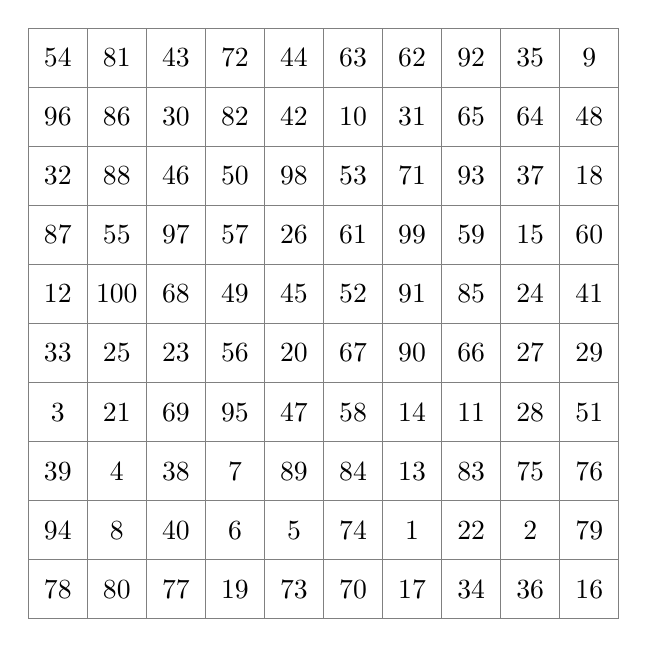
\begin{tikzpicture}[scale=0.75]
	\randintlist[min=1,max=100,nb=100]{\mylistsquare}
	\draw[thin,gray] (0,0) grid (10,10) ;
	\foreach \i in {1,...,100}{%
		\xdef\tmpnumber{\getitemfromrandintlist{\mylistsquare}{\i}}%
		\xdef\tmpnumberrow{\xinteval{\xintiiRem{\i-1}{10}}}%
		\xdef\tmpnumbercol{\xinteval{\xintiiQuo{\i-1}{10}}}%
		\draw ({0.5+\tmpnumbercol},{0.5+\tmpnumberrow}) node {\tmpnumber} ;
	}%
\end{tikzpicture}
\end{DemoCode}

\pagebreak

\section{History}

\texttt{0.1.4: Bugfix}

\texttt{0.1.3: Bugfix}

\texttt{0.1.2: Changing name of internal macro}

\texttt{0.1.1: Possibility to exclude values}

\texttt{0.1.0: Initial version}

\section{The code}

\DemoCodeFile{randintlist.sty}

\end{document}
